\centerline{\bf I. Introduction}
\addcontentsline{toc}{subsection}{I. Introduction}
\smallskip

\rory{get 'er done!}

\bigskip
\centerline{\bf II. Objectives and Significance}
\addcontentsline{toc}{subsection}{II. Objectives and Significance}
\smallskip

\rory{What is the point}.

\bigskip
\centerline{\bf III. Technical Approach and Methodology}
\addcontentsline{toc}{subsection}{III. Technical Approach and Methodology}
\smallskip

\medskip
{\centerline{\ub{\sc Transit Duration}}}
\smallskip

What is this definition?  Center of planet crossing?

\begin{eqnarray}
\Delta t_{circ} & = & {{P}\over{\pi}}~{{\sqrt{R_*^2 - b_0^2}}\over{a}} \nonumber \\
                & = & {{P}\over{\pi}}~{{\sqrt{1 - \beta_0^2}}\over{\alpha}}
\label{eq-tcirc}
\end{eqnarray}
where $P$ is the orbital period in cgs units, $R_*$ the stellar radius
in cgs, $b_0$ the minimum planetary impact parameter in cgs, $\beta_0$
a unitless measure of the minimum impact parameter (scaled by the
stellar radius), $a$ the planetary semi--major axis in cgs, and
$\alpha$ this value scaled by the stellar radius.


\medskip
{\centerline{\ub{\sc Fitted Transit Model}}}
\smallskip

To avoid a dependency between the fitted model and a physical model
that includes orbital dynamics, we parameterize the fitted lightcurve
in purely geometric terms.  To do so, we adopt the quadratic
limb--darkened model of \cite{2002ApJ...580L.171M}, which describes
transit lightcurves in terms of two (nuisance) limb--darkening
coefficients and two (important) system parameters.  The first of the
system parameters is the planetary radius divided by the stellar
radius ($\zeta \equiv Rp/R_*$), which determines the fractional area
of the stellar disk that may be occulted by the planet.  The second is
the impact parameter of the planet ($\beta \equiv b/R_*$).  This
variable is a function of time due to the objects' relative motion.
This function is dependent on the chord that the planet takes across
the stellar disk, itself typically estimated using the orbital
parameters semi--major axis and inclination.

Instead we use here a purely geometric parameterization, represented
in Figure~\ref{fig-schem}.  We describe the impact parameter as a
function of time using the minimum impact parameter $\beta_0$ -- when
the centers of the sources are aligned along the x--axis at
center--of--transit time $t_0$ -- and the location of the planet on
the transit chord across the stellar disk.  The x--coordinate of the
planet as a function of time is represented as $x(t) / R_* = (t - t_0)
* v_\perp / R_* = (t - t_0) / \tau$, where $v_\perp$ is the (unknown)
perpendicular velocity, and $\tau$ is the (fitted) amount of time it
takes the planet to traverse a distance equal to the stellar radius
assuming no acceleration.  This allows us to express geometrically the
impact parameter as a function of time:
\begin{eqnarray}
\beta(t) & = & \sqrt{\beta_0^2 + \left((t - t_0) / \tau\right)^2},
\end{eqnarray}
which is then used along with $\zeta$ to generate a model transit
lightcurve.

The transit duration $\Delta t$ may be found from the 2 solutions to
$\beta(t) = 1$, and represents the time between the center of the
planet crossing each limb of the star:
\begin{eqnarray}
\Delta t & = & 2 * \tau \sqrt{1 - \beta_0^2}.
\label{eq-dt}
\end{eqnarray}
This model yields a 4--parameter fit to each transit: $t_0, \beta_0^2,
\tau, \zeta$.  The system period $P$ may be determined using the
ensemble of $t_{0;i=1...N}$.

Combining Equation~\ref{eq-dt} with Equation~\ref{eq-emin}, we express
$e_{min}$ in terms of our model parameters:
\begin{eqnarray}
e_{min} & = & \pm \frac{P^{2} - 4 \pi^{2} \alpha^{2} \tau^{2}}{P^{2} + 4 \pi^{2} \alpha^{2} \tau^{2}}
\label{eq-emin2}
\end{eqnarray}
All factors of the minimum impact parameter $\beta_0$ cancel out,
which is fortuitous as this is typically the least constrained of all
system parameters, especially for the long--cadence Kepler data.
While the uncertainty in $\beta_0$ will affect our knowledge of the
other system parameters, this uncertainty may be marginalized out by
examining the posterior distributions, and drives us to use
Markov--Chain Monte Carlo (MCMC) modeling (described below).

Equation~\ref{eq-emin2} indicates that $e_{min}$ is purely a function
of the fitted parameter $\tau$, the derived period $P$, and an assumed
semi--major axis for the planet (in units of the stellar radius)
$\alpha$.  The uncertainty in $e_{min}$ scales as below for all 3
parameters:

\begin{eqnarray}
\Xi & \equiv & \frac{16 \pi^{2} \alpha^{2} \tau^{2} P^{2}}{16 \pi^{4} \alpha^{4} \tau^{4} - P^{4}} \\
\frac{\delta e_{min}}{\delta \xi} & = & \frac{\Xi~e_{min}}{\xi} ~~~~~ \left[\xi = \tau; P; \alpha \right].\nonumber
\label{eq-emin3}
\end{eqnarray}
In the limit of a circular orbit ($P \rightarrow 2 \pi \alpha \tau$),
$\Xi~e_{min}$ = 1.

\begin{figure*}[t] 
  \begin{minipage}[c]{0.37\textwidth}
    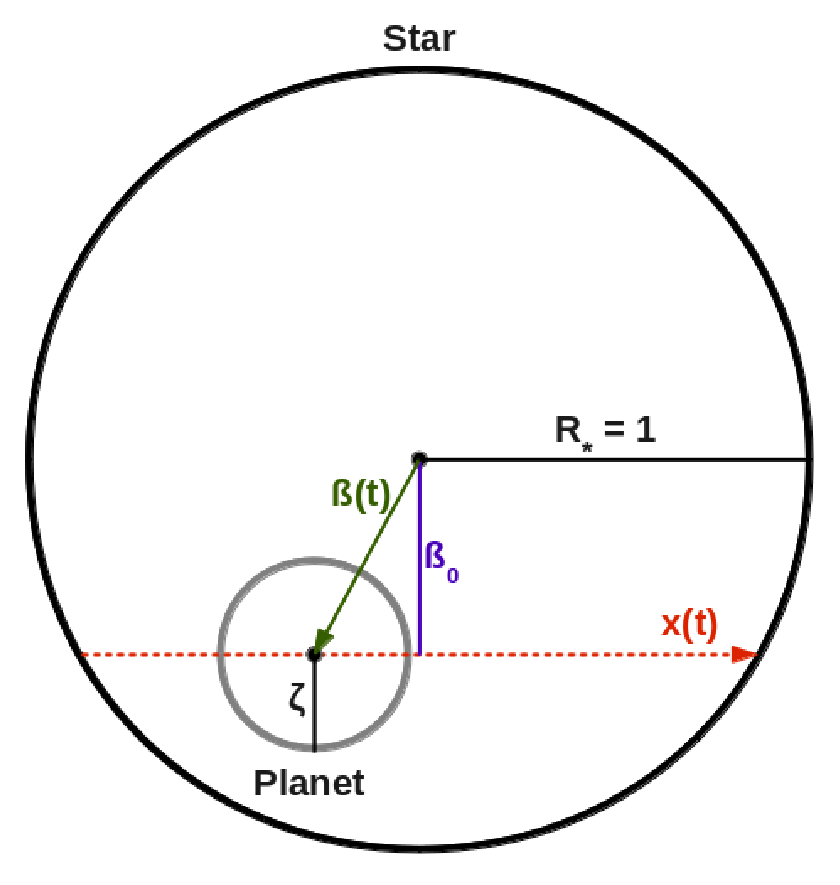
\includegraphics[width=\textwidth]{figures/schem.eps}
  \end{minipage}\hfill
  \begin{minipage}[c]{0.6\textwidth}
    \caption{Schematic detailing our geometric model for the impact
      parameter as a function of time, $\beta(t)$.  Relevant variables
      include the minimum impact parameter scaled by the stellar radius
      $\beta_0$, the radius of the planet scaled by the stellar radius
      $\zeta$, and the time-dependent position of the planet $x(t)$.  The
      fitted parameters are $t_0$ (defined where $\beta(t_0) = \beta_0$),
      the minimum impact parameter $\beta_0$, scaled planetary radius
      $\zeta$, and $\tau$ (which represents the time for the planet to
      travel the angular distance subtended by the stellar radius). }
    \label{fig-schem}
    \hspace*{\fill}  
    \hrule
  \end{minipage}
\end{figure*}

\medskip
{\centerline{\ub{\sc Simulations}}}
\smallskip

\rory{Describe the fake systems}

We use the system inclination, semi--major axis, planet--to--star
radius ratio, and period (along with two limb darkening parameters) to
generate fake system lightcurves using the method of
\cite{2002ApJ...580L.171M}.  The system lightcurve is evaluated once
each minute and integrated over 30 evaluations to approximate a single
Kepler long--cadence observation.  This is done for a window of 1 day
on either side of the given transit midpoint to ensure significant
out--of--transit data to include in the fit.  We perform these
evaluations for all transits for 14 ``quarters'' of Kepler
observations, or approximately 1280 days.

A white--noise component is added to each lightcurve for each of 4
magnitude bins, using the precisions in parts--per--million (ppm)
given on the Kepler calibration
webpage \footnote{http://keplergo.arc.nasa.gov/CalibrationSN.shtml}.
We evaluate each lightcurve separately for magnitude 8/10/12/14
objects, adding a random contribution of amplitude 11.3/29/80/296 ppm
(respectively) to each datapoint as generated above.  We do not
include red noise, or other transient gaps and features known to exist
in the Kepler data.  This yields a set of 4 lightcurves per simulated
system, each having hundreds of individual transits to fit.

\medskip
{\centerline{\ub{\sc KOI 701.01}}}
\smallskip

We validate the results of our simulations by analyzing Kepler data
from KOI 701.01 \citep[Kepler 62--b;][]{2013arXiv1304.7387B}.  This
planet has a period of 5.715 days, $\zeta = 0.018$ (R$_p$ $\sim$ 1.3
R$_E$), and a transit depth of $4 \times 10^{-4}$~\%.  We use the limb
darkening parameters for the host star from
\cite{2010A&A...510A..21S}.  The Kepler data have correlated noise
that is not included in our simulated data above, which is an
additional complication to the analysis.  To account for this, we
perform a local detrending by first dividing the data by the proposed
model, and fitting a low order spline to the result.  The goodness of
fit is determined by comparing the product of the spline and the model
to the data.  Figure~\ref{fig-koi70101} provides an example model fit
determined in this manner.  The data used are the {\tt PDCSAP} fluxes
and uncertainties.

\begin{figure*}[t] 
  \begin{minipage}[c]{0.6\textwidth}
    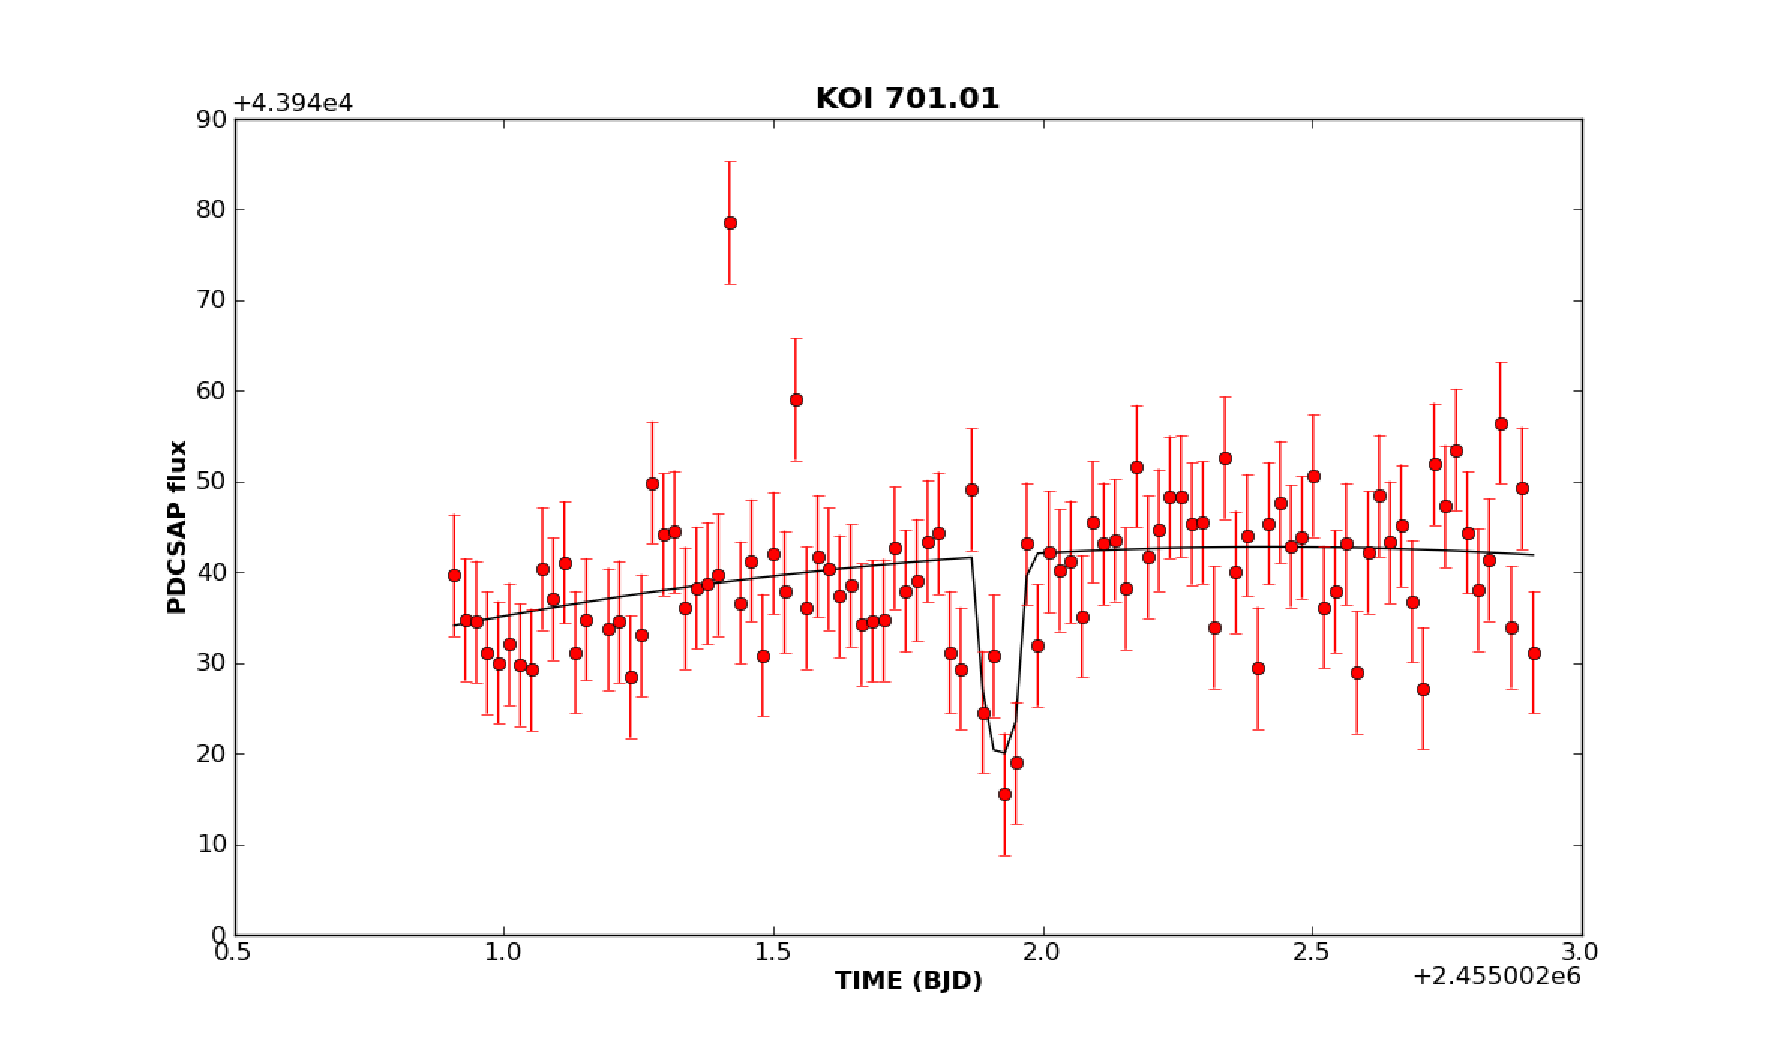
\includegraphics[width=\textwidth]{figures/701.01.eps}
  \end{minipage}\hfill
  \begin{minipage}[c]{0.4\textwidth}
    \caption{An example of our local detrending algorithm, applied to
      the first transit of KOI 701.01.  The data and model (solid
      line) are in {\tt PDCSAP} flux units.  The solid curve is
      generated by first dividing the data by the transit model,
      applying a low--order spline to the normalized data, and then
      taking the product of the spline and the model.}
    \label{fig-koi70101}
    \hspace*{\fill}  
    \hrule
  \end{minipage}
\end{figure*}

\medskip
{\centerline{\ub{\sc Model Evaluation}}}
\smallskip

To examine how our knowledge of system parameters evolves as a
function of number of transits, we have fit {\it all} the data up to
the time of each transit, for all $N$ transits in each lightcurve.
This means that for transit $n \leq N$, we have common model
parameters $\beta_{0}^2, \tau, \zeta$ and per--transit parameters
$t_{0;i=1..n}$, for a total of $n+3$ model parameters.  This yields an
ensemble of $N$ system models per lightcurve, each incorporating one
more transit than the previous one.

We use the affine--invariant MCMC sampler {\tt emcee}
\citep{2013PASP..125..306F} to sample the posterior distribution of
the model parameters.  This program uses the method of
\cite{Goodman-Weare} to achieve high sampling performance independent
of the aspect ratio of the posterior distribution, meaning covariances
between parameters are less important to the efficacy of the MCMC
sampling.  This provides a set of MCMC chains that we examine to
determine our constraints on the fitted parameters.  We use the
Gelman--Rubin $\hat{\rm R}$--static \citep{Gelman92} to assure that
each chain sufficiently samples model space, and require effective
chain lengths larger than $10^4$ to ensure sufficient mixing in the
MCMC sample \cite[e.g.][]{2004PhRvD..69j3501T}.  Our trial runs using
KOI 701.01 indicate that our chains typically have autocorrelation
lengths of $\sim 100$, requiring a total number of steps per chain of
$10^6$.  This may be achieved by using a set of $N$ {\tt emcee}
``walkers'', each taking $10^6/N$ steps.  We use burn--in times having
10\% the requested number of steps, which are then discarded before
the final chain commences.

For each transit, we evaluate the joint and marginalized distributions
of $\zeta$ and $\tau$.  Figure~\ref{fig-joint} demonstrates how the
joint distribution evolves from fitting 1 transit (dashed contours,
which represent 68.3\%, 95.5\%, and 99.7\% confidence limits), to
fitting all transits (solid contours, at the same confidence limits),
for KOI 701.01.  We then marginalize over all other parameters, and
examine the per--parameter confidence limits.  Figure~\ref{fig-marg}
demonstrates how our marginalized constraints on $\zeta$ (left panel)
and $\tau$ (right panel) evolve as a function of the number of
transits used in the fit for 701.01.  The solid line provides the
maximum of the posterior distribution, and the dashed line indicates
its median.  The shaded area encloses 68.3\% of the distribution.  In
this way we quantify $\delta \tau$, as this is necessary to understand
our ability to constrain $e_{min}$ via Equation~\ref{eq-emin3}.

\begin{figure*}[t] 
  \begin{minipage}[c]{0.47\textwidth}
    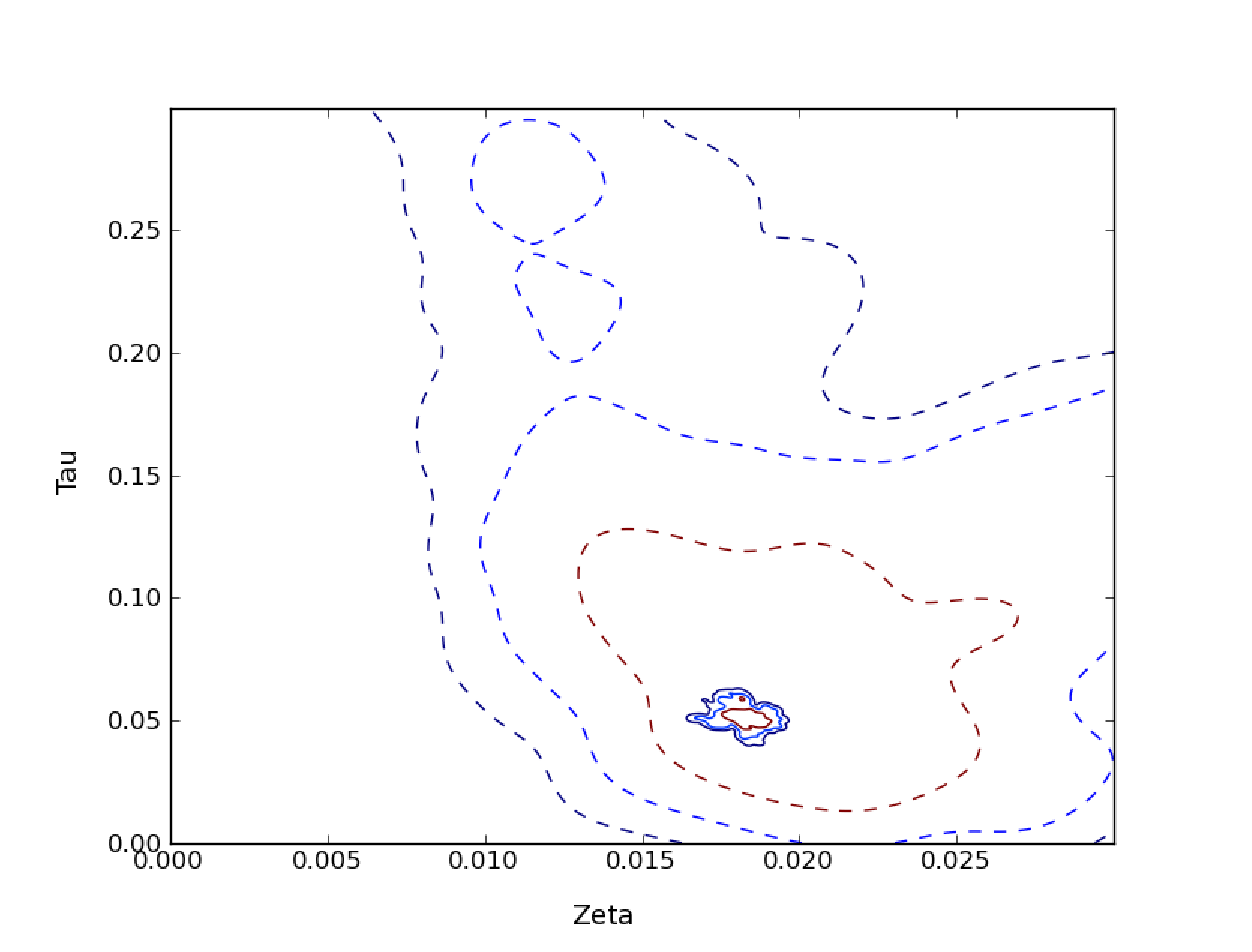
\includegraphics[width=\textwidth]{figures/joint.eps}
  \end{minipage}\hfill
  \begin{minipage}[c]{0.5\textwidth}
    \caption{The joint distribution of $\zeta$ vs. $\tau$ for KOI
      701.01.  The {\it dashed} lines show the distribution when
      fitting 1 transit, with contours at the 68.3\%, 95.5\%, and
      99.7\% confidence limits.  The {\it solid} lines show the
      distribution when fitting $N$ transits simultaneously.}
    \label{fig-joint}
    \hspace*{\fill}  
    \hrule
  \end{minipage}
\end{figure*}


\begin{figure*}[t] 
\begin{center} 
\mbox{
\subfigure{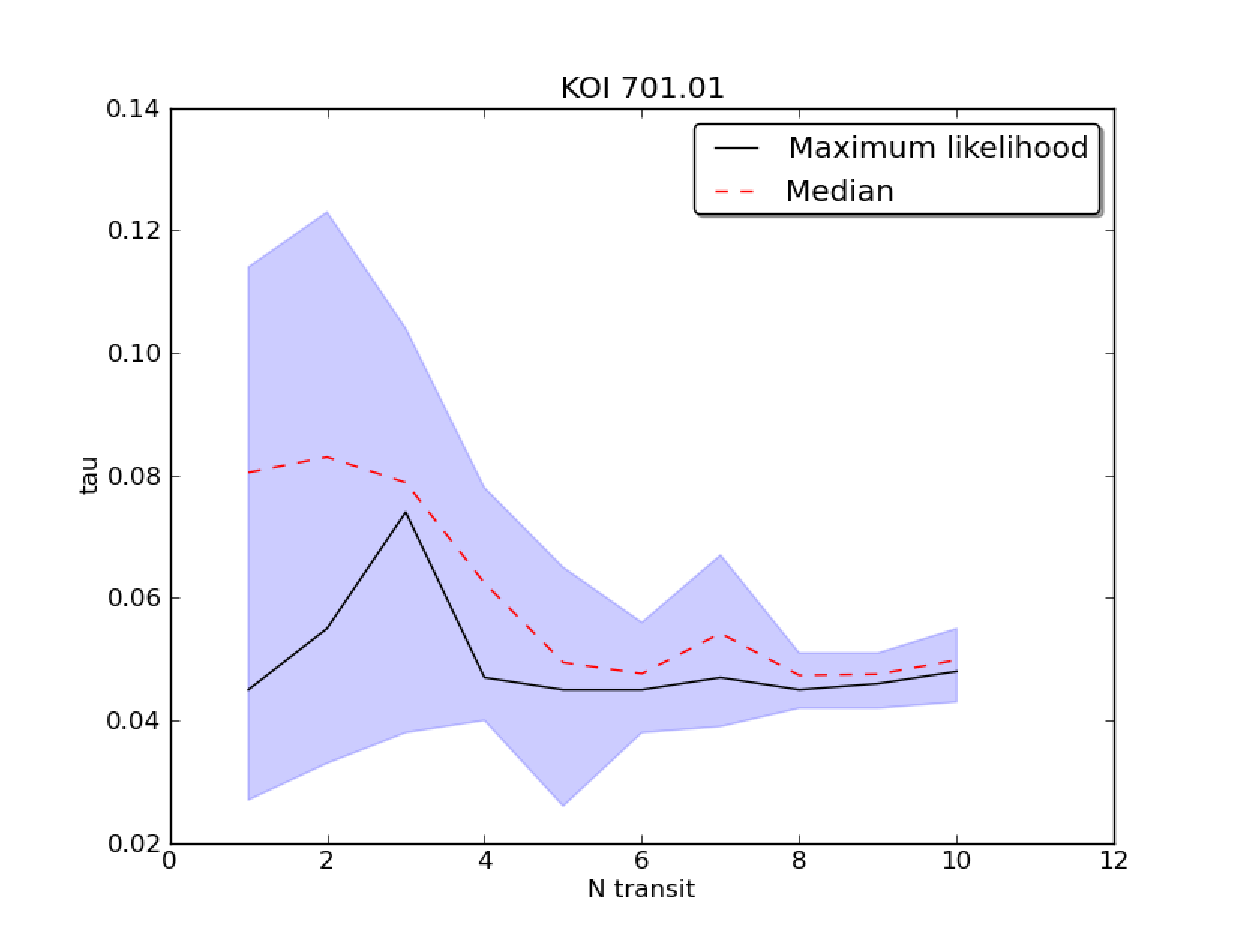
\includegraphics[width=0.47\textwidth]{figures/tau.eps}}
\quad
\subfigure{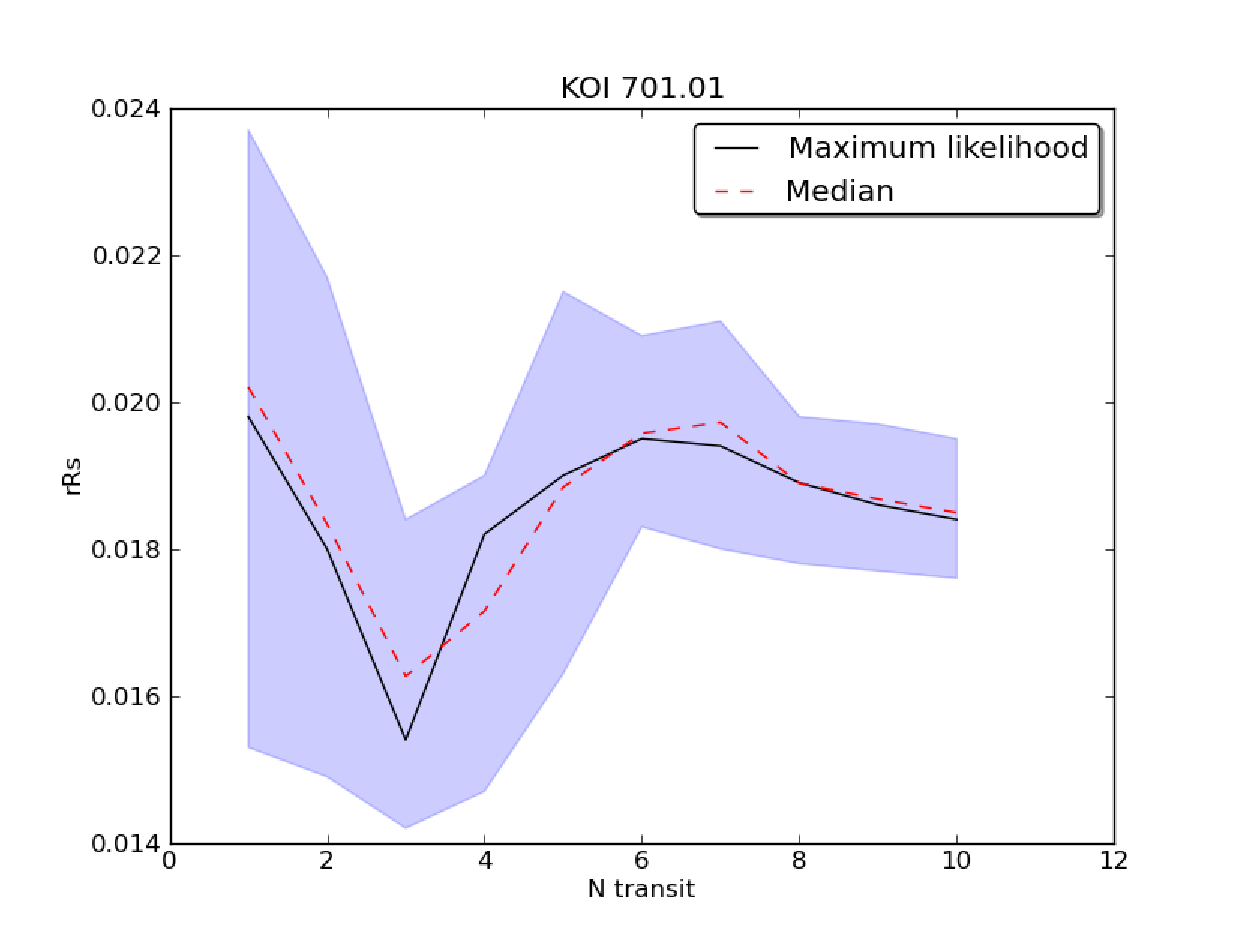
\includegraphics[width=0.47\textwidth]{figures/rRs.eps}}
}
\caption{The marginalized distributions of $\tau$ (left panel) and
  $\zeta$ (right panel) as a function of the number of transits being
  used, for KOI 701.01.  For each transit $n \leq N$ we use {\it all}
  data up to and including transit $n$ to constrain $\zeta$ and $\tau$
  (along with $\beta_0^2$ and times of transit $t_{0;i=1...n}$).  The
  {\it solid} line represents the maximum of the posterior
  distribution, while the {\it dashed} line indicates its median.  The
  shaded area contains 68.3\% of the posterior samples.}
\hspace*{\fill}  
\hrule
\label{fig-marg} 
\end{center} 
\end{figure*}

To examine our constraints on the system period, we use the
$t_{0;1..n}$ posterior distributions from the fits described above.
We use {\tt emcee} to sample the posterior space of (nuisance
parameter) $t_{0;1}$ and period $P$.  For a given trial ($t_{0;1}, P$)
pair, the likelihood is determined through:
\begin{eqnarray}
\mathcal{L}(t_{0;1}, P) & = & \prod_{i=1}^{i=n} \kappa_i(t_{0;1} + P * (i-1))
\end{eqnarray}
where $\kappa_i$ is a kernel density estimate of each posterior
distribution $t_{0;i}$, which is evaluated at the predicted time of
transit $t_0 + P * (i-1)$.  By modeling the times of transit
separately in the original MCMC analysis, we open the possibility of
using a more complex ephemeris model at this stage of the analysis,
such as may be expected from transit timing variations
\citep{2005MNRAS.359..567A,2005Sci...307.1288H}.  The results of this
analysis for KOI 701.01 are presented in Figure~\ref{fig-period}.

\begin{figure*}[t] 
  \begin{minipage}[c]{0.47\textwidth}
    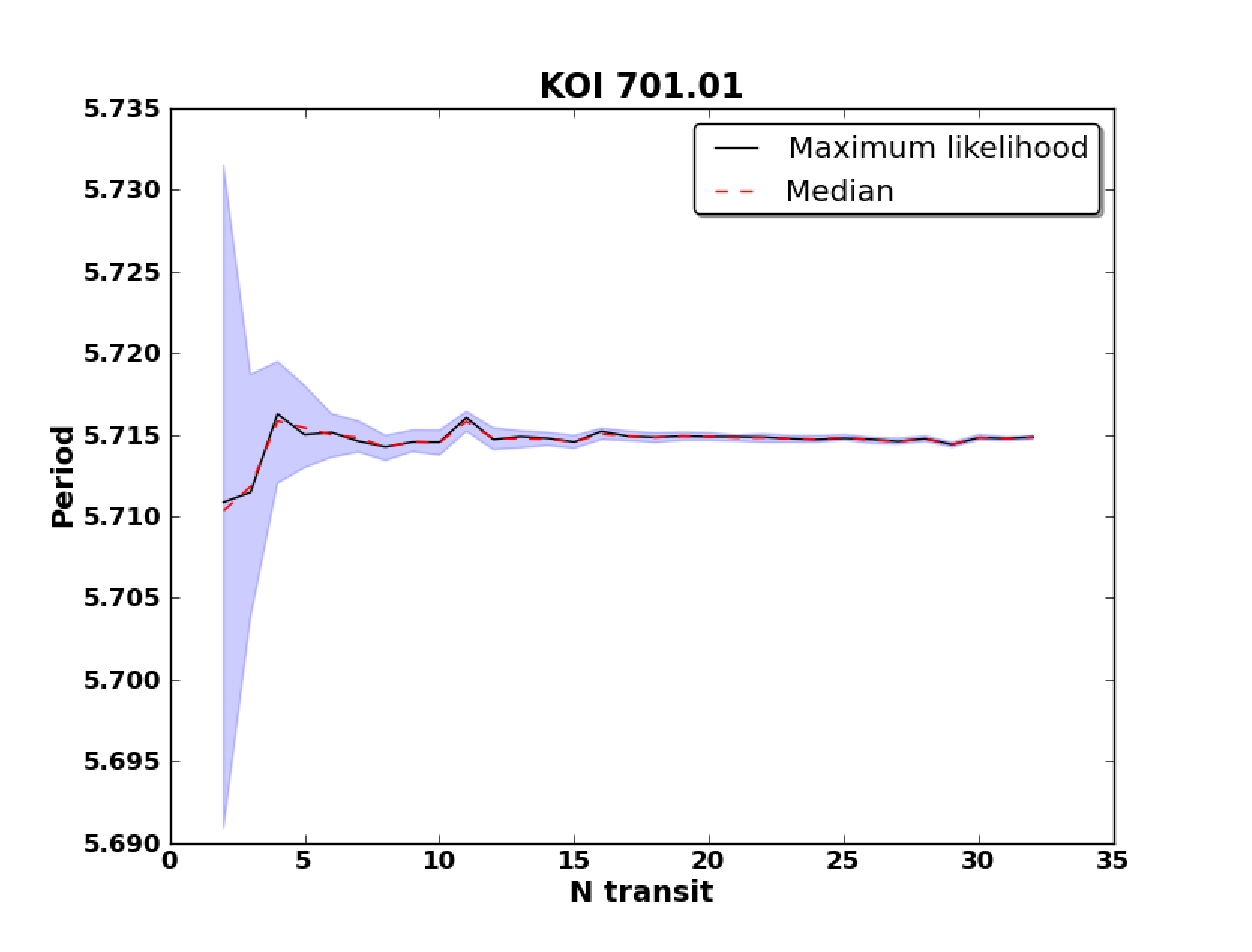
\includegraphics[width=\textwidth]{figures/period.eps}
  \end{minipage}\hfill
  \begin{minipage}[c]{0.5\textwidth}
    \caption{The evolution of the posterior distribution on orbital
      period $P$ (y--axis) based upon the results of modeling $n$
      times--of--transit (x--axis) separately.  The period posterior
      is generated by taking the product of the time--of--transit
      posteriors ($t_{0;i=1..n}$) evaluated at the predicted transit
      time $t_0 + P * i$, where $t_0$ is the (marginalized over) time
      of the first transit.  }
    \label{fig-period}
    \hspace*{\fill}  
    \hrule
  \end{minipage}
\end{figure*}


For our simulated data, Table~\ref{tab-taurun} lists the numbers of
transits that are needed to recover $\tau$ to 10\% as a function of
the system brightness and transit depth.

\begin{table}[t]
\begin{center}
\caption{\label{tab-taurun} Number of transits needed to recover $\tau$ to 10\%}
\begin{tabular}{c|cccc}
\hline \hline
Transit Depth (\%) & Magnitude=8 & Mag=10 & Mag=12 & Mag=14\\
\hline
5e-5 & x & x & x & x \\
1e-4 & x & x & x & x \\
5e-4 & x & x & x & x \\
1e-3 & x & x & x & x \\
5e-3 & x & x & x & x \\
1e-2 & x & x & x & x \\
\hline
\end{tabular}
\end{center}
Estimates of the number of transits needed to recover the value of
$\tau$ to 10\%, based on our simulated systems.  We determine this as
a function of transit depth, and the signal--to--noise of the
lightcurve (here, determined solely by the host star brightness).  We
combine all MCMC chains up to and including the transit listed here to
determine the multi--transit constraint on the distribution.
\hspace*{\fill} \\
\hrule
\end{table}

\medskip
{\centerline{\ub{\sc Kepler Sample Available for Analysis}}}
\smallskip

We need systems that are observed with the short cadence (ummm, maybe
not since we marginalize over $\beta_0$), are bright enough to resolve
$e_{min}$ to within 0.1, and have short period planets (less than 4
days).  From this sample, we will need to know the physical
characteristics of stellar mass and radius, and (ideally) age.

\medskip
{\centerline{\ub{\sc Computational Requirements}}}
\smallskip

Use KOI 701.01 as a benchmark

\bigskip
\centerline{\bf IV. Team Qualifications and Previous NASA Support}
\addcontentsline{toc}{subsection}{IV. Team Qualifications and Previous NASA Support}
\smallskip

PI Becker is PI on NASA OSS grant NNX09AB32G, ``3.5m Transit Timing
Observations at 100\% Duty Cycle'', which observed multiple transiting
exoplanet systems for evidence of transit timing variations
\citep{2011ApJ...731..123K, 2013ApJ...764....8K, 2013ApJ...764L..17B,
  2013arXiv1304.5713K}.  Much of the software developed for that
project has been modified to operate with the Kepler data, and used in
the analyses presented here.  He has considerable expertise in using
modern software packages implemented on distributed computing
infrastructures to model multi--dimensional systems.  Relevant
examples include the work done under NASA ADP grant NNX09AC77G, ``Time
Domain Studies of the 2MASS Calibration Point Source Working
Database'', for which he is also PI
\citep{2012ApJ...748...58D,2013ApJ...764...62D}.

Co--I Barnes...

Co--I Agol...

\bigskip
\centerline{\bf V. Relevance to NASA Programs}
\addcontentsline{toc}{subsection}{V. Relevance to NASA Programs}
\smallskip

This project addresses directly multiple objectives that are in--scope
for the Origins of Solar Systems call for proposals, including:
\begin{itemize}

\item {\bf Observations related to the formation and evolution of
  planetary systems}: Explain.

\item {\bf Theoretical investigations related to the formation and
  evolution of planetary systems}: Explain.

\item {\bf Characterization of extra-solar planets to explain
  observations of extra-solar planets}: Explain.

\item {\bf Characterization of extra-solar planets to improve
  understanding of the origins of planetary systems}: Explain.

\end{itemize}



\bigskip
\centerline{\bf VI. Project Development Plan}
\addcontentsline{toc}{subsection}{VI. Project Development Plan}
\smallskip

PI Becker will be technical lead the project for the first 1.5 years,
which will constitute the data analysis (MCMC) portion of the project.
He will work at 50\% FTE with the graduate student to implement the
computations on the Kepler sample of data.  Co--I Barnes will serve as
technical lead for the project for the second 1.5 years, as the
project transitions from analysis of the data to interpretation and
constraints on tidal evolution theory.  Co--I Agol has significant
experience in dealing with the Kepler data, including implementing
detrending algorithms to correct for correlated noise in the Kepler
data.  He will advise as--needed throughout the project.  PI Becker
will serve as the project lead throughout.

We regard the professional development of students as an important
responsibility of {\it any} research project.  In this regard, the
graduate students funded by this proposal will have the opportunity to
attend at least one relevant conference each year, and encouraged to
give oral presentations on our work.  This will become a requirement
as the project progresses.  We expect the graduate student to become
an expert in both areas of this project, both the
computational/modeling side and the theoretical side.  This student
will receive a strong dose of both data and theory, which is a
powerful combination and one not seen often enough in the field.  We
consider this dual--aspect training a strong component of this
project.

{\bf Year 1 (2014):} This first year of the project will start with PI
Becker bringing the student up to speed in modeling transit
lightcurves, in leaning Bayesian techniques, and in implementing a
robust application of the {\tt emcee} package (or other
affine--invariant sampler, if needed).  Making the software robust to
detrending errors, missing data, and initial conditions for the
samplers is a non--trivial exercise.  Discovering and understanding
the failure modes will be a main focus of this first
computationally--intensive first year.  Becker will lead this effort,
and transition the student into lead during the year.  The generation
of the MCMC chains is expected to take {\tt XXX} CPU--hours, or {\tt
  YYY} calendar--hours on {\tt ZZZ}. The validation of these chains
(Gelman--Rubin $\hat{\rm R}$ and effective chain lengths) is expected
to take a comparable amount of time, as some chains are expected to
have to be re--run or extended.  The goal of this first year is to
have finalized the MCMC chains on $t_0, \beta_0^2, \tau, \zeta$ for
all transits of all KOIs.  We will make these publicly available
through a {\tt github} site specifically designed for this project.
Our modeling software will also be released via {\tt github}.

{\bf Year 2 (2015):} The second year is expected to begin with the
MCMC analyses of the periods via times of transit, and transition to
theoretical interpretation of the systems.  We will start with linear
ephemeris models for all systems to estimate periods; for those
systems where this model is insufficient, we will examine transit
timing models with more complicated ephemerides.  We anticipate that
this effort will result in the publication of 1 or more ancillary
papers on the transit timings of the systems under study, with
assistance from Agol on the interpretation of the results.  We then
hand off to \rory{XXX}.

{\bf Year 3 (2016):} 
\rory{XXX}

\bigskip
\centerline{\bf VII. Data Sharing Plan}
\addcontentsline{toc}{subsection}{VII. Data Sharing Plan}
\smallskip

All investigators are committed to the sharing of data and software.
PI Becker has been behind real--time public alert systems for many
time--domain astronomical surveys.  This includes the MACHO survey,
the Deep Lens Survey, the SuperMACHO and ESSENCE surveys, and the
SDSS--II Supernova Survey, all of which have released their events to
the public in near--real time through web pages, Astronomer's
Telegrams, IAU circulars, and VOEvents.  He has been diligent in
releasing the software and data behind publications.  This includes
the image subtraction software {\tt hotpants}, period finding software
{\tt Supersmoother}, and spatial clustering software {\tt
  OPTICS}\footnote{http://www.astro.washington.edu/users/becker/c\_software.html}
which have been used in many subsequent publications.  He is currently
working part--time on the Large Synoptic Survey Telescope (LSST),
which is both open--source and open--data.

We will version release all software developed for this project on the
publicly available open--source collaboration website
http://github.com ({\tt github} hereafter).  The website has become a
leading collaboration platform; it enables distributed users to
download code and contribute back to the project.  All code we develop
for this project will be made available under the terms of the open
source BSD
license\footnote{http://www.opensource.org/licenses/bsd-license.php}
whenever possible.  We will make a new {\tt github} account for this
project that we will use to stage code and data releases, as described
in the project development plan.  Analysis packages used in our
publications will be released as {\tt
  iPython}\footnote{http://ipython.org} notebooks to help establish
reproducible research standards in the field.


